\documentclass[conference]{IEEEtran}
% \IEEEoverridecommandlockouts
% The preceding line is only needed to identify funding in the first footnote. If that is unneeded, please comment it out.
\usepackage{cite}
\usepackage{amsmath,amssymb,amsfonts}
\usepackage{algorithmic}
\usepackage{graphicx}
\usepackage{textcomp}
\usepackage{xcolor}
\usepackage{hyperref}
\def\BibTeX{{\rm B\kern-.05em{\sc i\kern-.025em b}\kern-.08em
    T\kern-.1667em\lower.7ex\hbox{E}\kern-.125emX}}

\graphicspath{{./images/}}

\begin{document}

\title{Real-Time Road Sign Detection and Classification\\
}

\author{\IEEEauthorblockN{1\textsuperscript{st} Dumitru Mițca}
\IEEEauthorblockA{\textit{dept. CTI} \\
\textit{Technical University "Gheorge Asachi" of Iași}\\
Iași, Romania \\
dumitru.mitca@student.tuiasi.ro}
\and
\IEEEauthorblockN{2\textsuperscript{nd} Mihai Mihalache}
\IEEEauthorblockA{\textit{dept. CTI} \\
\textit{Technical University "Gheorge Asachi" of Iași}\\
Iași, Romania \\
mihai.mihalache2@student.tuiasi.ro}
\and
\IEEEauthorblockN{3\textsuperscript{rd} Otilia Zvorișteanu}
\IEEEauthorblockA{\textit{dept. CTI} \\
\textit{Technical University "Gheorge Asachi" of Iași}\\
Iași, Romania \\
otilia.zvoristeanu2@academic.tuiasi.ro}
\and
\IEEEauthorblockN{4\textsuperscript{th} Simona Caraiman}
\IEEEauthorblockA{\textit{dept. CTI} \\
\textit{Technical University "Gheorge Asachi" of Iași}\\
Iași, Romania \\
simona.caraiman@academic.tuiasi.ro}
}

\maketitle

\begin{abstract}
Road signs are a vital part of traffic infrastructure and their correct detection and classification
is a vital task in autonomous driving applications. In this paper, we present a cursory study over
state-of-the-art software solutions and related papers in the field, and then we present our initial
implementation of such an application.
\end{abstract}

\begin{IEEEkeywords}
computer vision, road sign detection, autonomous driving
\end{IEEEkeywords}

\section{Introduction}
Road sign detection and classification is a significant task in the computer vision space, that
has been studied for at least a decade and a half. Applications in this domain have strict requirements,
as mistakes or software bugs can lead to significant financial loss or even human death in the worst case,
requirements such as:
\begin{itemize}
    \item low, tending towards 0\%, misclassification rate --- classifying a stop sign as a right-of-way
    sign can lead to accidents, this example is unlikely to happen in a real application, but it shows
    the worst case scenario; more likely missclassication would be "must go left" as "must go right", or
    misclassifying the various "road thins ahead" signs between each other
    \item high speed --- a vehicle should not stop at every road sign it encounters in order to recognize it
    then proceed, abiding its instructions, this process should be real-time
    \item high tolerance to bad weather conditions --- fog, rain and snow are very common conditions in
    various parts of the world, an autonomous vehicle should be able to function correctly in any of these
    conditions. This point ties into the low missclassification rate point
    \item high tolerance to bad lightning --- similar to the above
    \item low hardware cost --- cars are already expensive, by including expensive high resolution cameras
    or expensive processors to run the detection and classification steps, the costs would be very unreasonable
    for the vast majority of people
\end{itemize}

\begin{figure}
    \centerline{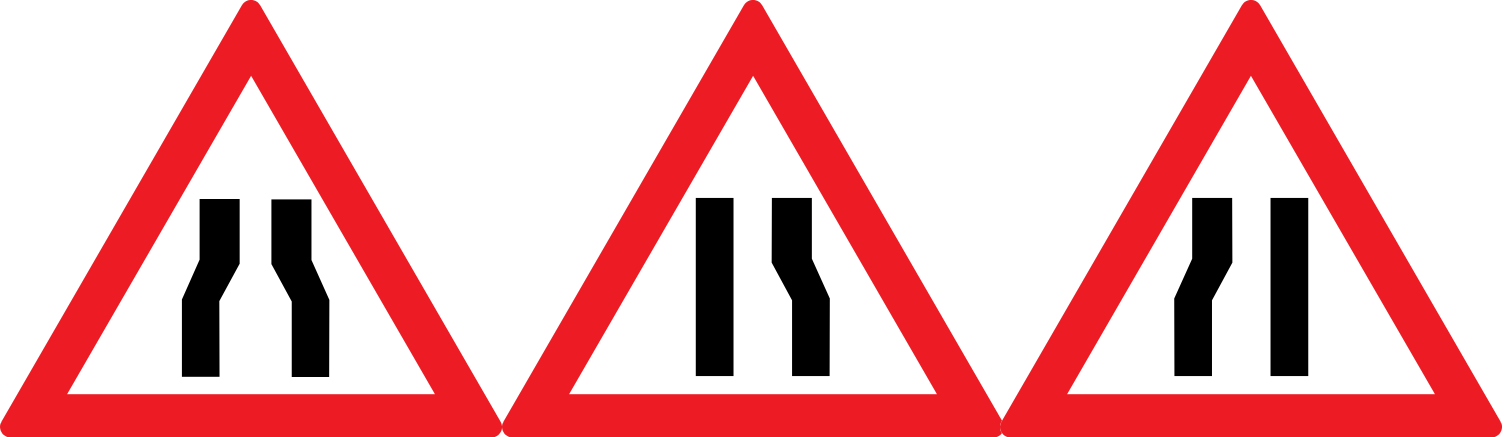
\includegraphics[width=\linewidth]{confusables}}
    \caption{Three confusable signs, in order from left to right: "Îngustarea șoselei din ambele sensuri",
    "Îngustarea șoselei din dreapta", "Îngustarea șoselei din stânga"\protect\footnotemark}
\end{figure}

\footnotetext{By Gigillo83, own work CC BY-SA 4.0, \url{https://commons.wikimedia.org/w/index.php?curid=40362644},
\url{https://commons.wikimedia.org/w/index.php?curid=40362647}, \url{https://commons.wikimedia.org/w/index.php?curid=40362645},
stitched by Mițca Dumitru into a single image.}

\subsection{Related work}
We've surveyed a number of papers in this domain in order to discover what approach we should follow in our
own application.

Reference \cite{4370763} was interesting to read but ultimately we found the approach in this paper
to be limiting as it could only detect road signs with red borders that were either circles or triangles.

Reference \cite{Karthika2022} proposed an approach that had multiple layers of preprocessing before
the detection and classification itself, which was done using the YOLO architecture.

Reference \cite{metastudy2019}, a metastudy on the state of computer vision in traffic sign detection and
recognition in 2019, was very useful as it showed us approaches that would be likely be useful
with good accuracy and clear paths to take in development. It confirmed to us that an approach where
the detection and recognition steps were split was a good idea as it is what most of the literature
surveyed did. We initially believed that we could use grayscale datasets to simplify our machine learning
(ML) models, but \cite{metastudy2019} infirmed this belief showing us that colour-based approaches would
have higher accuracy. Reference \cite{4290244} claims that a grayscale approach would be based on shape
detection and be computationally expensive.

We approached \cite{8709983} due to its generic title, but it is an application in traffic sign inventory
management, and as such has less strict requirements than our application, and a much higher error rate
is acceptable in its domain.

Reference \cite{6196571} presents an approach where the detection of road signs is done using classical
segmentation methods, while the recognition itself is done using a multilayer perceptron neural network.

Conclusions:
\begin{itemize}
    \item this kind of application should be split in two big modules: a detection module and a
    recognition module, with any number of pre-processing before them
    \item the detection module can be implemented using classical methods, while the recognition
    module must be implemented using neural networks
    \item grayscale approaches are not computationally viable
\end{itemize}



\subsection{State of the art}

For existing software solutions we surveyed the pretrained YOLOv8 model YOLOv8n and ...

Through experimentation using the pretrained YOLOv8 model, we came to the conclusion that pretrained
models are unlikely to be useful to particular applications, due to the pretrained models' generality
and datasets where weather and or lightning conditions aren't varied enough.

\begin{figure}[h!]
    \centerline{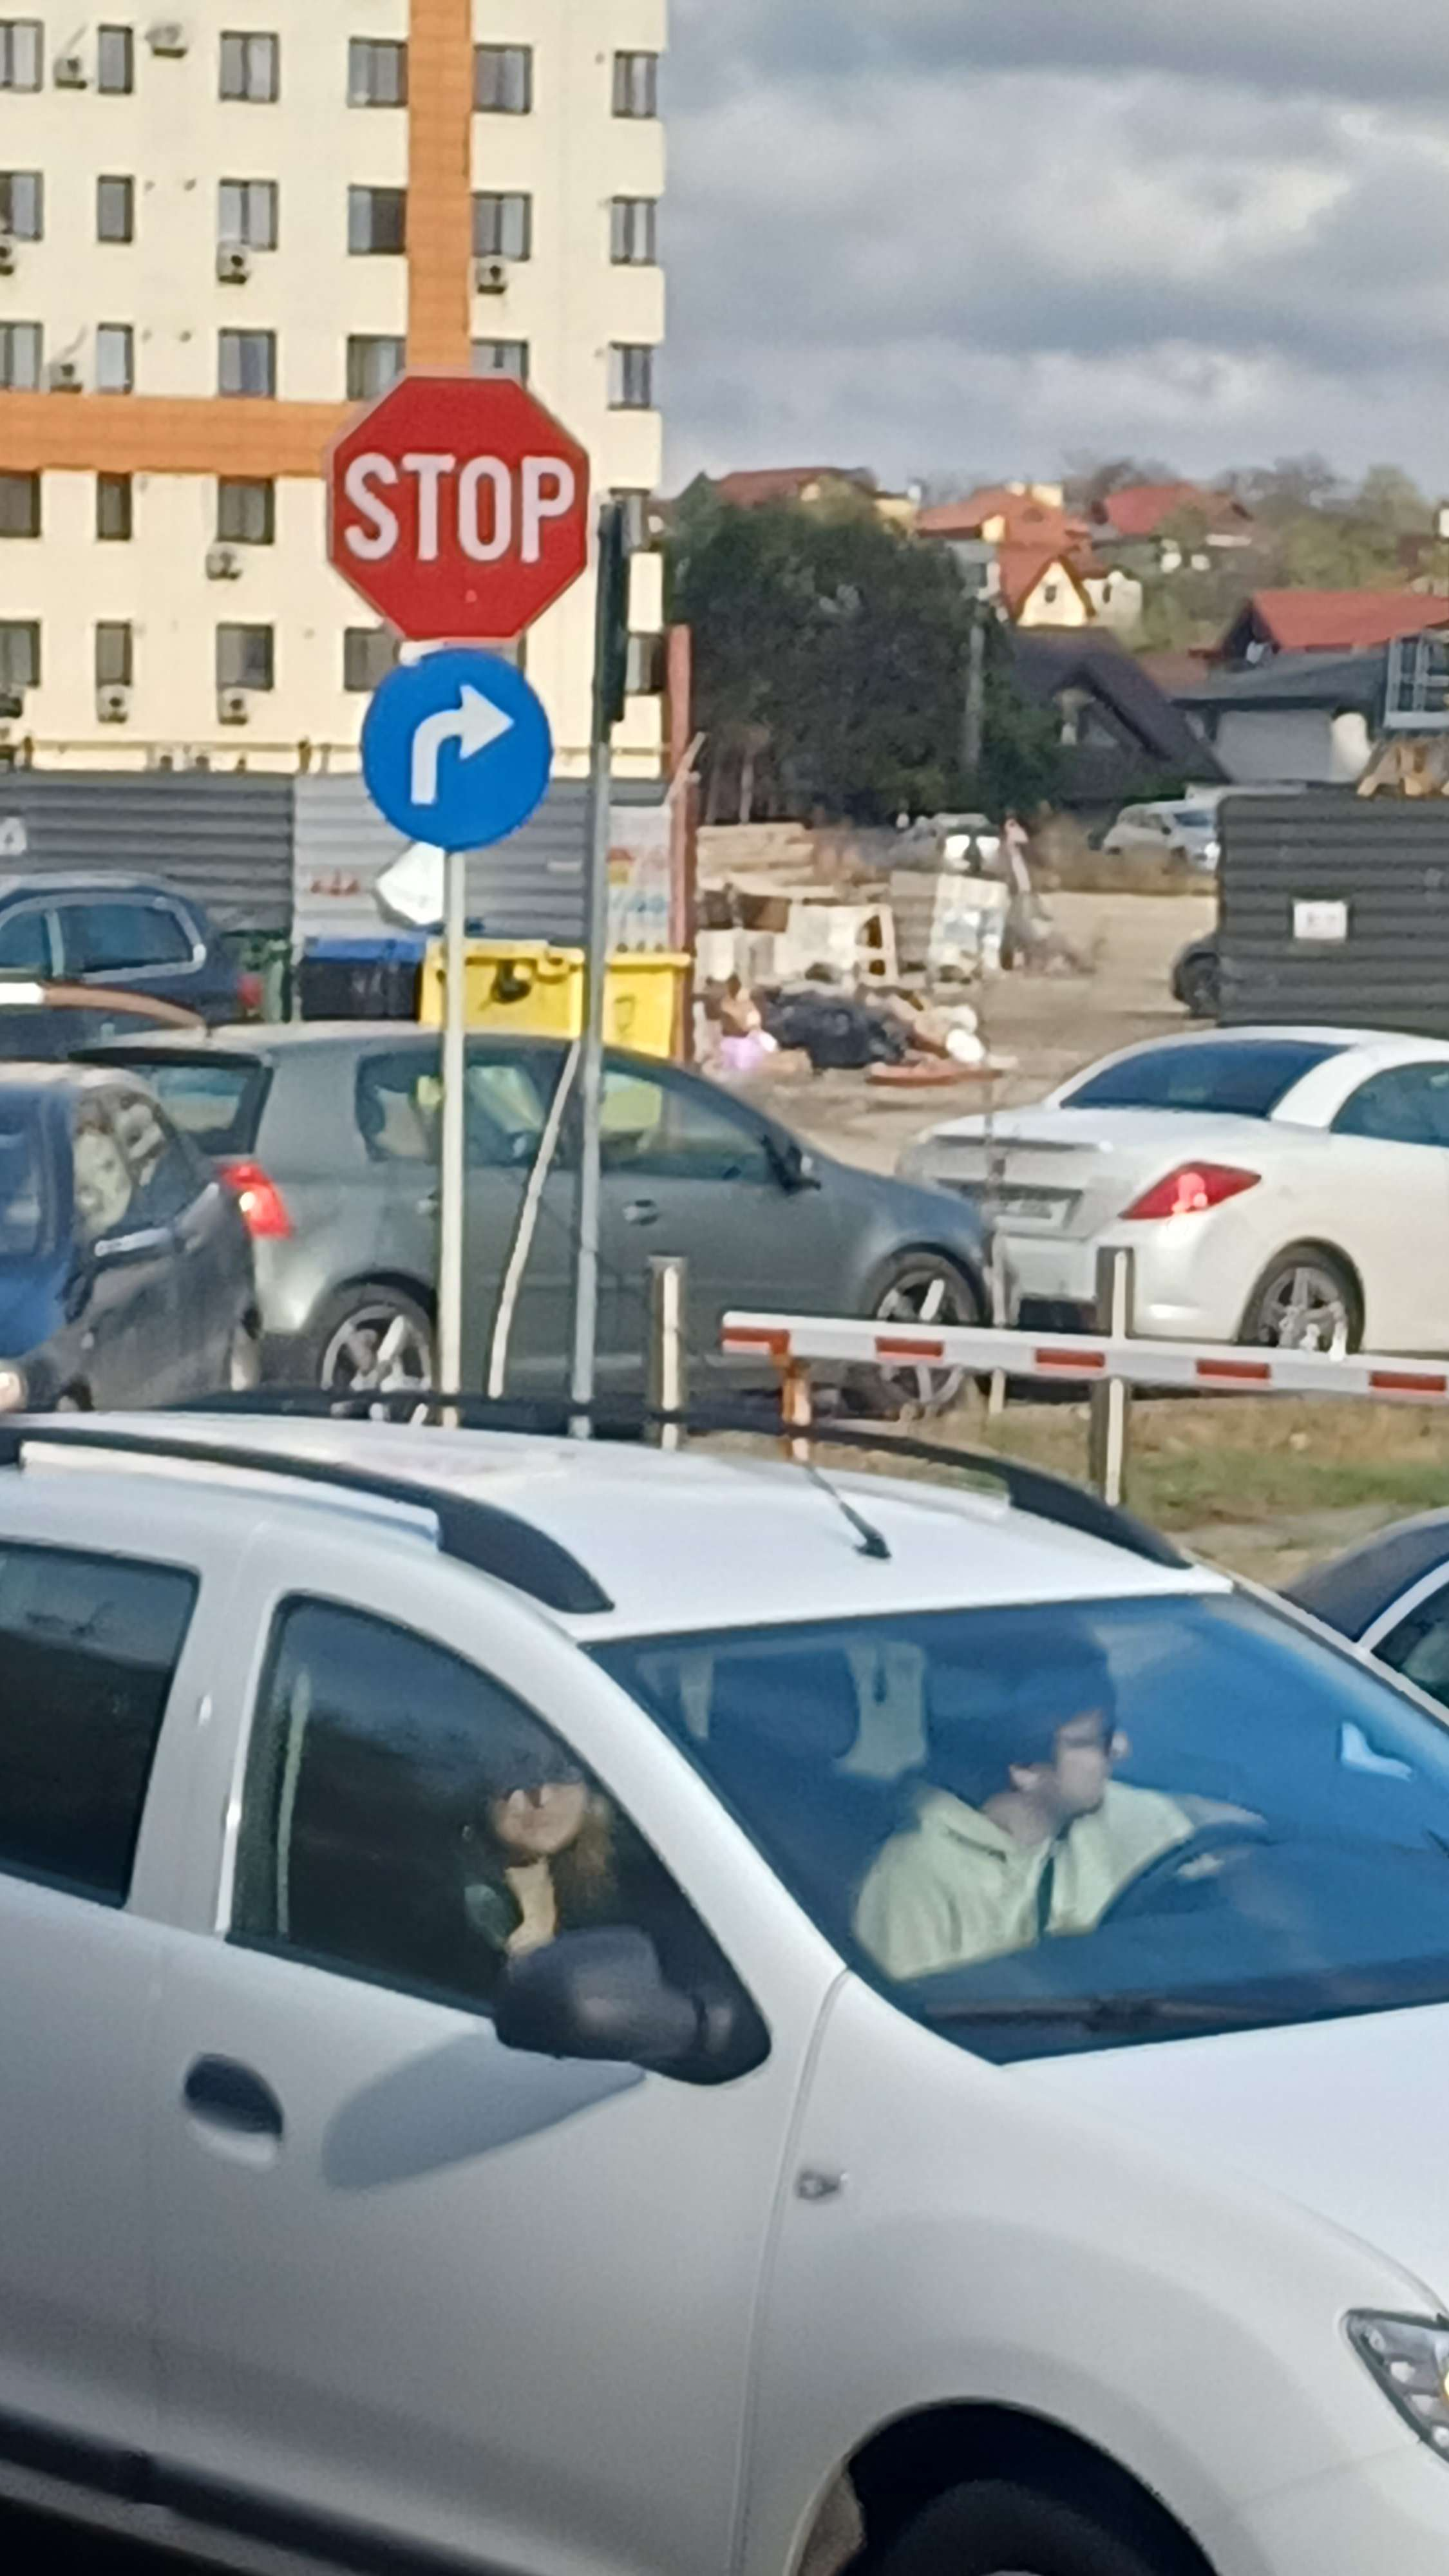
\includegraphics[width=0.5\linewidth,]{poza-fata-ac}}
    \caption{YOLOv8n with no additional training detects 2 stop signs in this image}
\end{figure}

\section{Method description}

We propose an approach in which the process is split in two steps, following existing practices:
a sign detection step and a sign recognition step.

\bibliographystyle{IEEEtran}
\bibliography{IEEEabrv,refs}
\end{document}
